\documentclass{article}
\usepackage{scrextend}
\usepackage[dvips,a3paper,centering,margin=2cm]{geometry}
\usepackage{multirow}
\usepackage[spanish]{babel}
\usepackage{framed}
\usepackage{xcolor}
\usepackage{color}
\definecolor{shadecolor}{rgb}{0.8431,0.8627,0.8470}
\usepackage[spanish, english]{babel} 
\usepackage[utf8]{inputenc}
\usepackage{amsmath}
\definecolor{rb}{rgb}{0.025,0.5,0.9} 
\definecolor{na}{rgb}{0.8274,0.305,0.196} 
\definecolor{ver}{rgb}{0.0823, 0.4705, 0.1411}
\usepackage{graphicx}  
\pagestyle{empty}
\def\to{\rightarrow}
\begin{document}
\vspace*{-2cm}
\changefontsizes{14pt}
\hspace*{-1cm}
\begin{minipage}{0.2\linewidth}
\vspace{0.7cm}
\vspace*{-0.15cm}
\includegraphics[scale=0.12]{images/ifir.eps}
\end{minipage}
\vspace*{-0.4cm}
\begin{minipage}{0.65\linewidth}
\vspace*{0.7cm}
\begin{center}
\changefontsizes{15pt}
\hspace*{-0.1cm}
\textbf{\textcolor{ver}{Estudio de la irradiancia solar con dos modelos de transferencia radiativa y su comparación con mediciones en la cuidad de Monterrey}}
\end{center}
\vspace{-1cm}
\begin{center}
\changefontsizes{11pt}
Gamaliel López-Padilla$^1$, Adriana Ipiña$^{*2}$,Martín Freire$^{2,3}$,Benedetto Schiavo$^{4}$ Rubén Piacentini$^{2,3}$\\
1. Facultad de Ciencias Físico-Matemáticas,UANL, México\\
2. Instituto de Física Rosario,CONICET-UNR, Argentina\\
3. Facultad de Ciencias Exactas Ingenieria y Agrimensura, UNR, Argentina\\
4. Centro de Ciencias de la Atmósfera, UNAM, México\\
email: giovannilopez9808@gmail.com, ipina@ifir-conicet.gov.ar
\end{center}
\end{minipage}
\begin{minipage}{0.2\linewidth}
\hspace*{0.2cm}

\includegraphics[scale=0.2]{images/fcfm.eps}
\end{minipage}
\vspace{0.2cm}
\changefontsizes{12pt}
\begin{center}
\begin{shaded}
\textbf{\textcolor{ver}{Introducción}}
\end{shaded}
\end{center}
\begin{minipage}{0.47\linewidth}
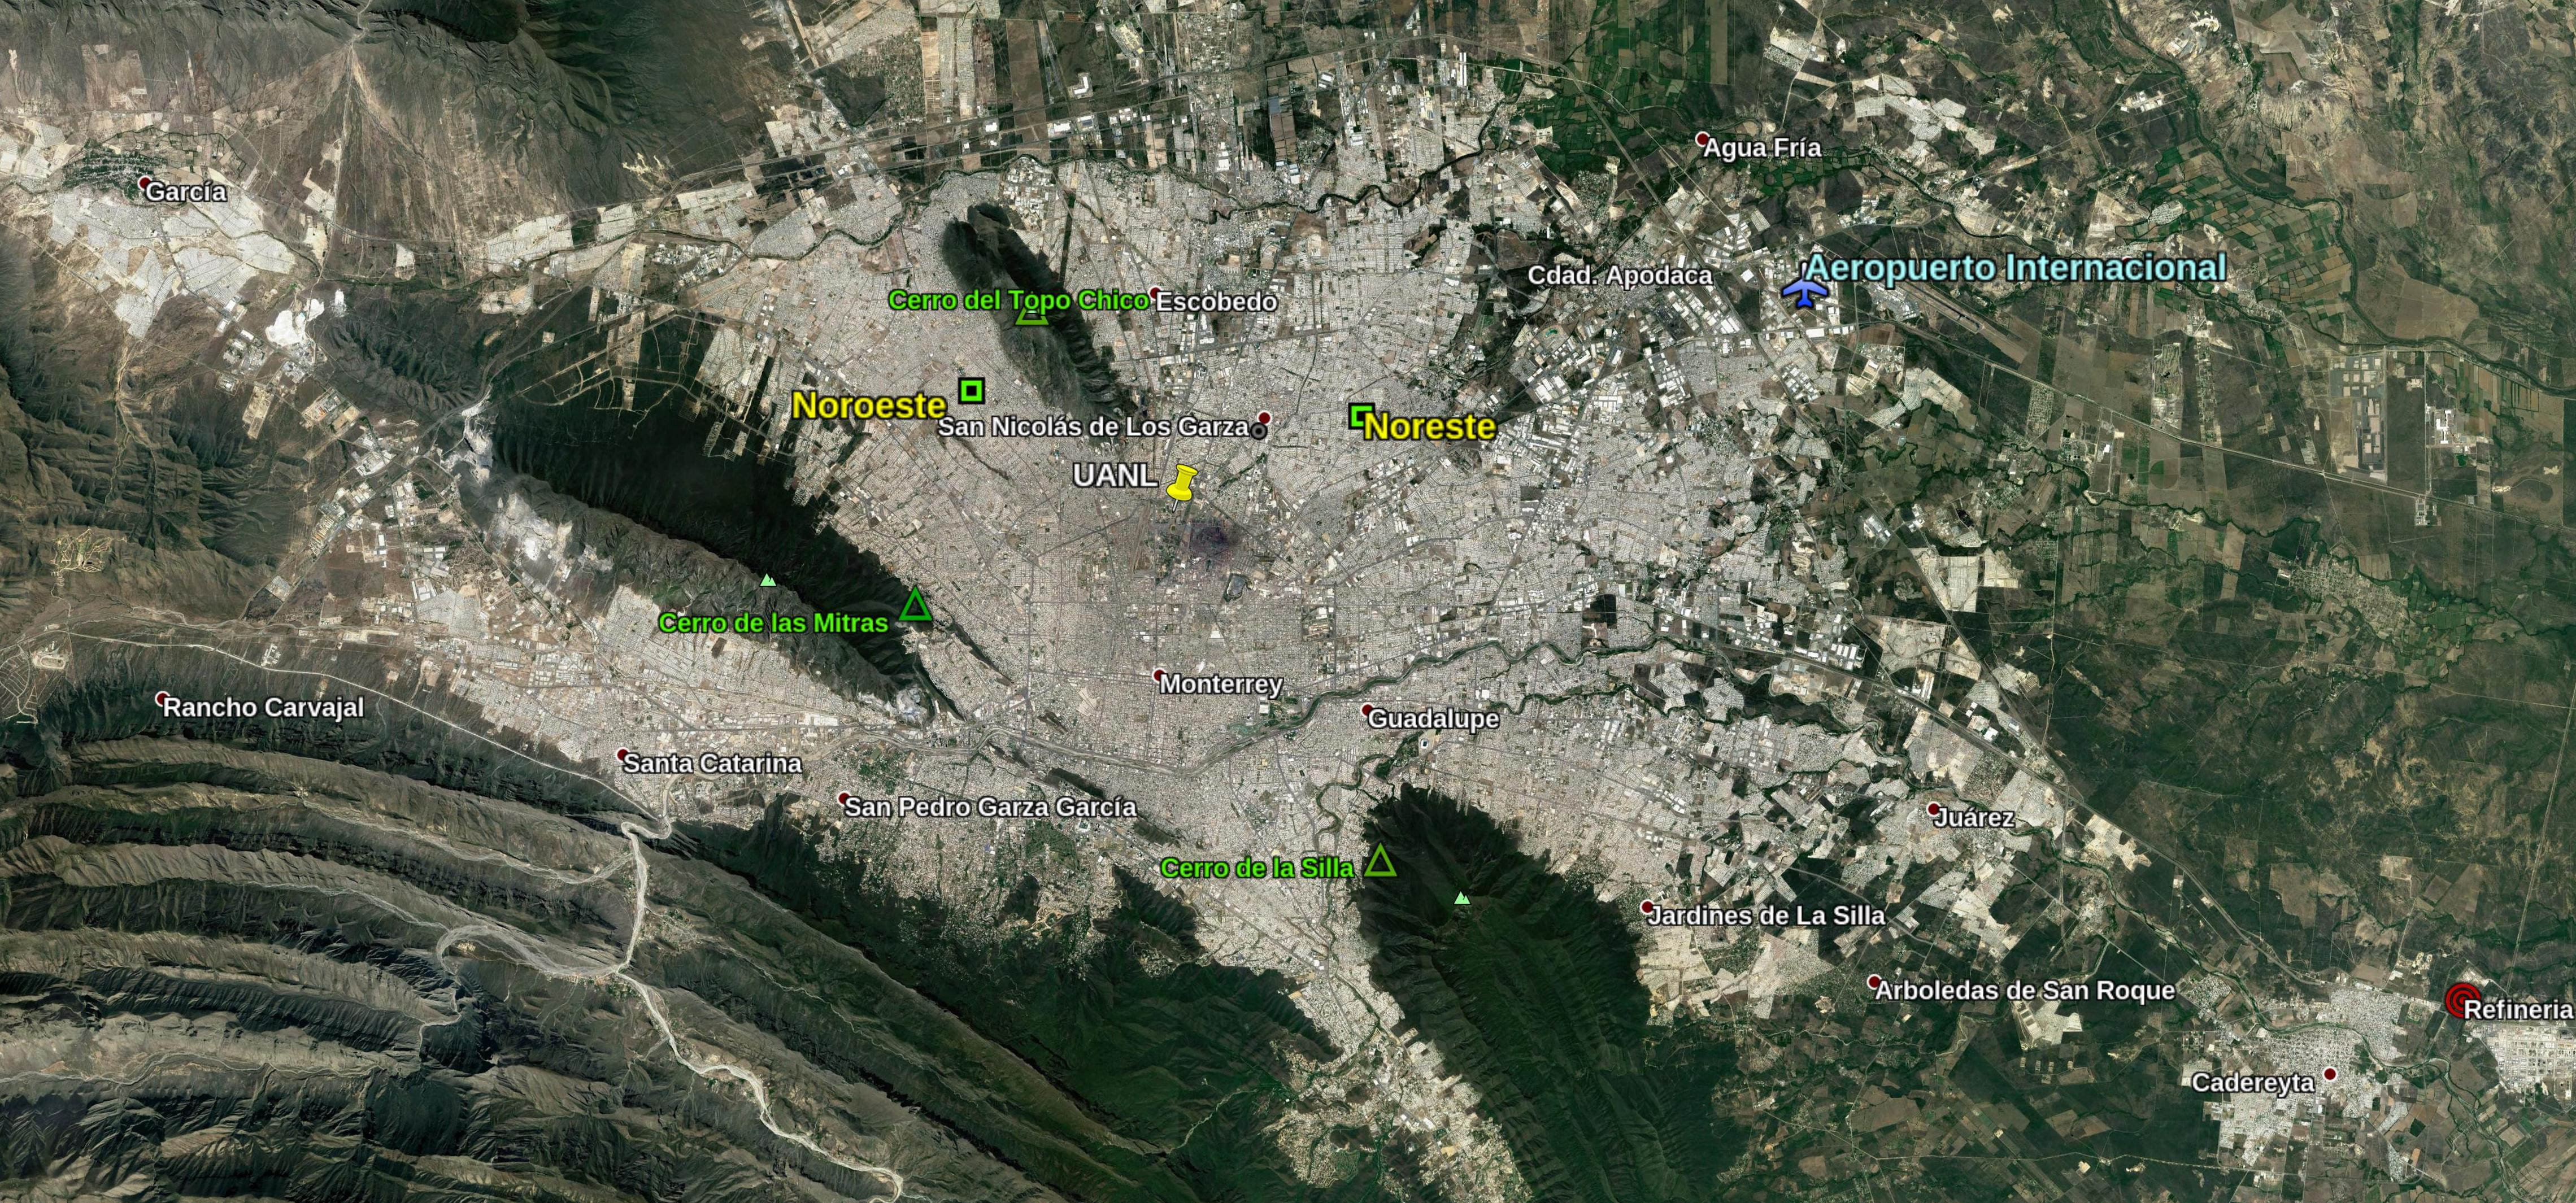
\includegraphics[scale=0.101]{images/satelite.jpg}\\
\end{minipage}
\hspace{-0.cm}
\begin{minipage}{0.53\linewidth}
Monterrey y su área metropolitana conforman la 3$^a$ región más poblada
de México y una de las de mayor deterioro en su Calidad del Aire en las últimas décadas. Por su ubicación geográfica y condiciones atmosféricas, la radiación solar alcanza niveles altos casi todo el año. Conocer la intensidad solar a nivel del suelo nos permite estimar los componentes que la atenúan y también evaluar sus efectos biológicos. Presentamos un análisis de la irradiancia solar Vis+NIR* medida en el periodo 2015-2018 en las estaciones Noreste (NE) y Noroeste (NO) del Sistema Integral de Monitoreo Ambiental (SIMA) de Nuevo León. Las mediciones bajo un cielo libre de nubes fueron las referencias para aproximación de los modelos TUV 5.3.2 y SMARTS 2.9.5$^{\left[1,2,3\right]}$.\\
\textbf{\textcolor{ver}{$\leftarrow$Imagen satélital del área metropolitana de Monterrey y
localización de estaciones Noreste y Noroeste del SIMA}}
\end{minipage} 
\begin{center}
\begin{shaded}
\textbf{\textcolor{ver}{Metodologia}}
\end{shaded}
\end{center}
\begin{minipage}{0.81\linewidth}
La irradiancia solar Vis+NIR* del SIMA se midió con un piranómetro MetOne096 de sensibilidad entre $\left[400,1100\right]$nm. De ellas se seleccionan días despejados en el periodo 2015-2018. Por otro lado, la Ecuación de Transferencia Radiativa:
\begin{equation*}
dL_{\lambda}=\sigma_e \ \left(z\right) \left(\cdots - \frac{\omega\left(z\right)}{4\pi} \left[I_{0\lambda}p\left(\vec{s*},\vec{s};z \right)exp\left(-\int\limits_z^\infty \frac{\sigma_e(z')}{cos\theta^*(z')}dz' \right)\cdots \int\limits_{4\pi}\int\limits_{4\pi} L_{\lambda}(\vec{s'};z)p(\vec{s'},\vec{s};z)d^2\omega' \right]\right)\frac{dz}{cos\theta}
\end{equation*}
es resuelta por los modelos SMARTS y TUV$^{\left[2,5\right]}$ para obtener la irradiancia solar espectral (L$_\lambda$). Cada modelo se ejecuta para una fecha y hora del día con los siguientes valores de entrada: 

\changefontsizes{9.5pt}
\begin{tabular}{|c|c|c|c|c|c|c|c|}
\hline
  Modelo & [Lat, Lon, a.s.n.m] NE/NO & Reflectividad  & O$_3$ col & NO$_2$ col DU & Exp. & Albedo de disp. & AOD$_{550nm}$ \\
  & & de suelo & & &Angström & simple de aerosol & \\ \hline
 TUV  & \multirow{2}{*}{25.75,-100.25,512m}& 0.06 & OMI-NASA DU & \multirow{2}{*}{0.1} & \multirow{2}{*}{1} & 0.87 & \multirow{2}{*}{(variable)$^{\left[4,5 \right]}$}\\ \cline{1-1}
SMARTS & & Concreto & OMI-NASA atm-cm &  &  & urbano & \\ \hline
\end{tabular}\vspace{0.2cm}\\
\changefontsizes{12pt}
Con un código propio se integró L$_\lambda$ entre $\left[400,1100\right]$nm para SMARTS y para TUV entre $\left[400,1000\right]$nm añadiendo una fracción aproximada a la integral en el rango espectral coincidente. Luego, la irradiancia Vis+NIR* se ajustó hasta que el AOD$_{500nm}$ logre una diferencia relativa (DR) $<$ 5\% al mediodía solar entre medición y modelo.
\end{minipage}
\hspace{0.3cm}
\begin{minipage}{0.18\linewidth}
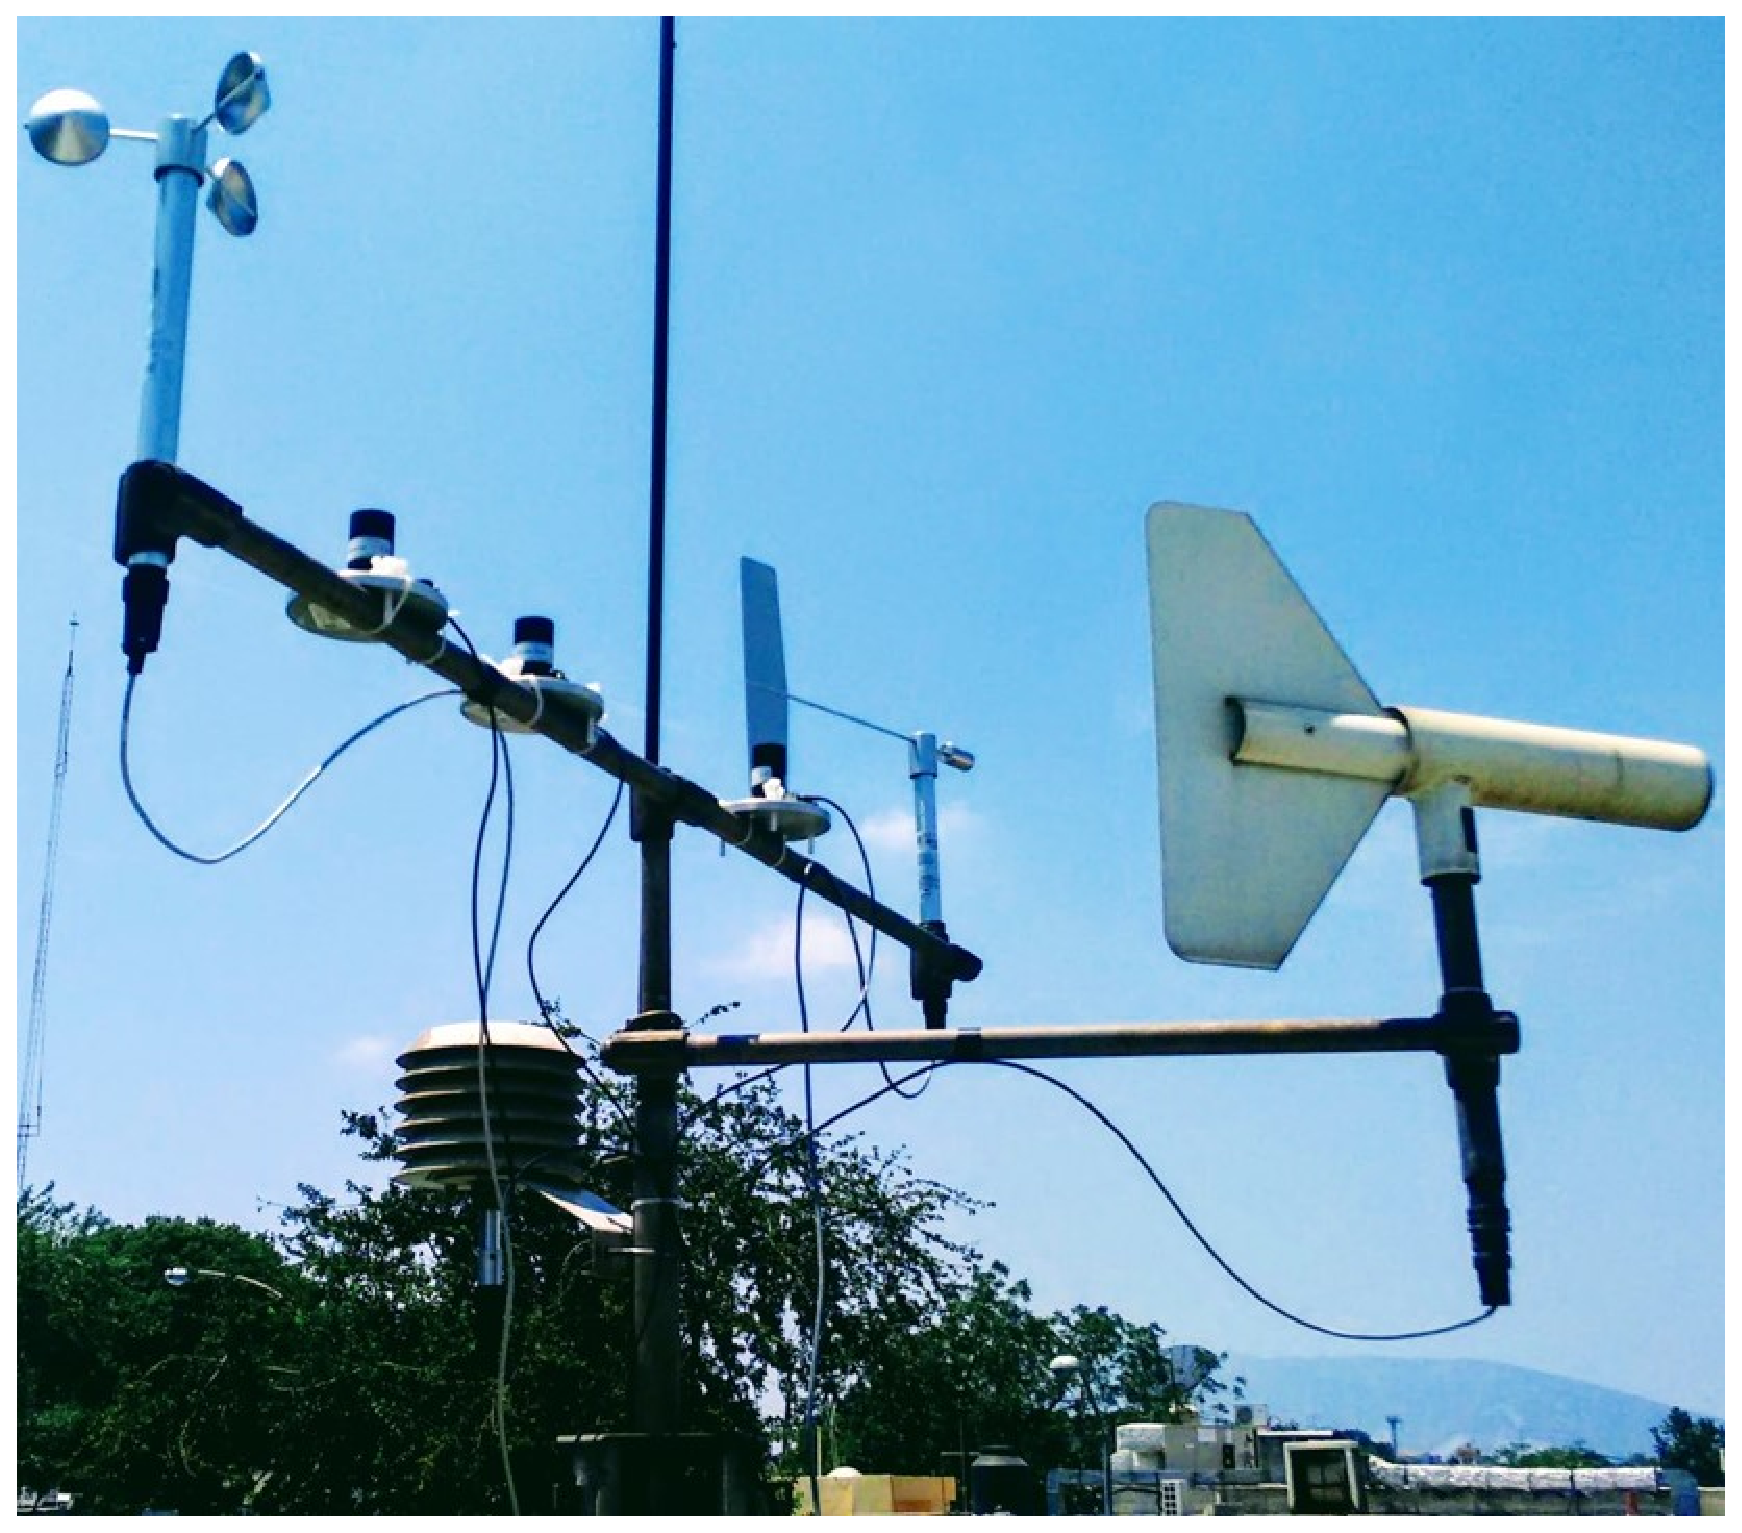
\includegraphics[scale=0.16]{instru.eps}
\begin{center}
\textbf{\textcolor{ver}{Instrumento de medición de la estación SIMA}}
\end{center}
\end{minipage}
\begin{center}
\begin{shaded}
\textbf{\textcolor{ver}{Resultados}}
\end{shaded}
\end{center}
\hspace{-1.3cm}
\begin{minipage}{0.53\linewidth}
\begin{minipage}{0.6\linewidth}
\includegraphics[scale=0.33]{images/espectro.eps}
\end{minipage}
\hspace{-0.4cm}
\begin{minipage}{0.4\linewidth}
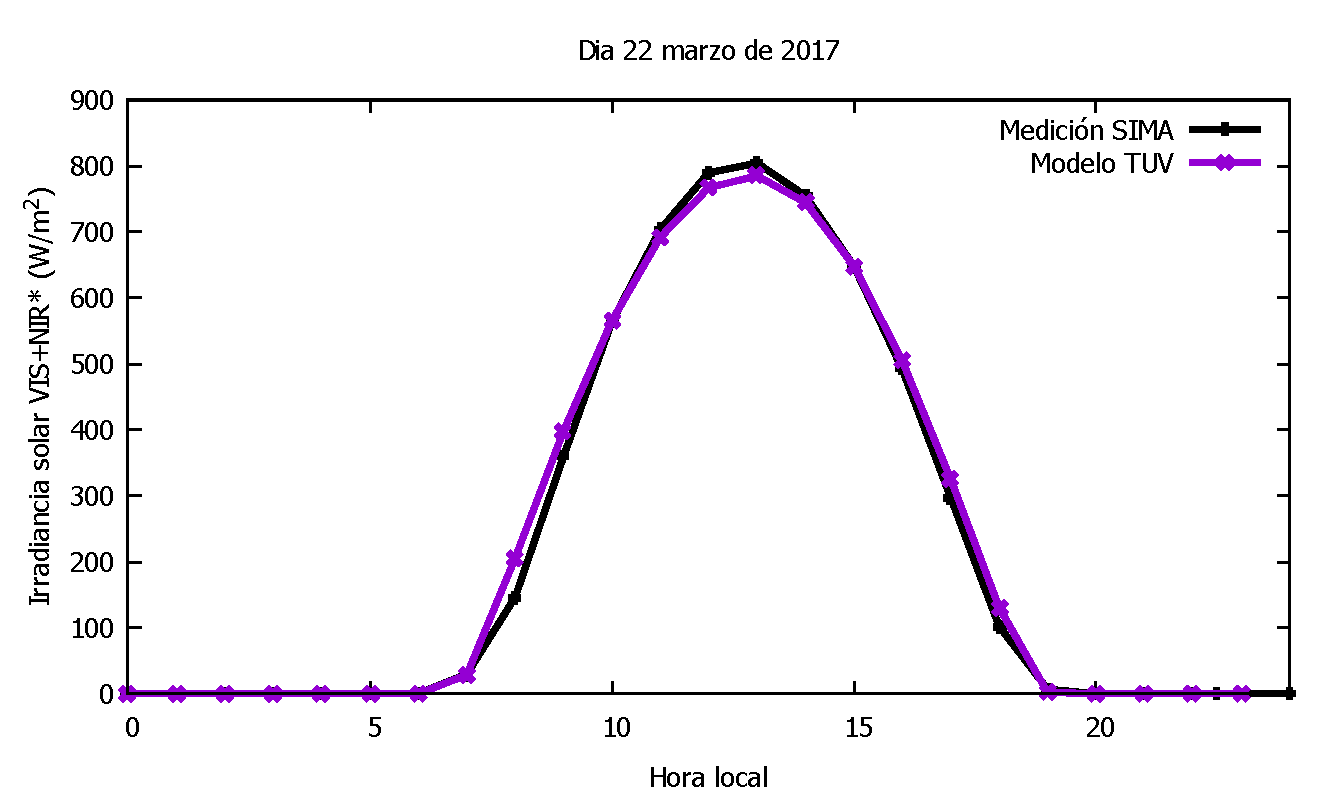
\includegraphics[scale=0.32]{images/med1.pdf}\\
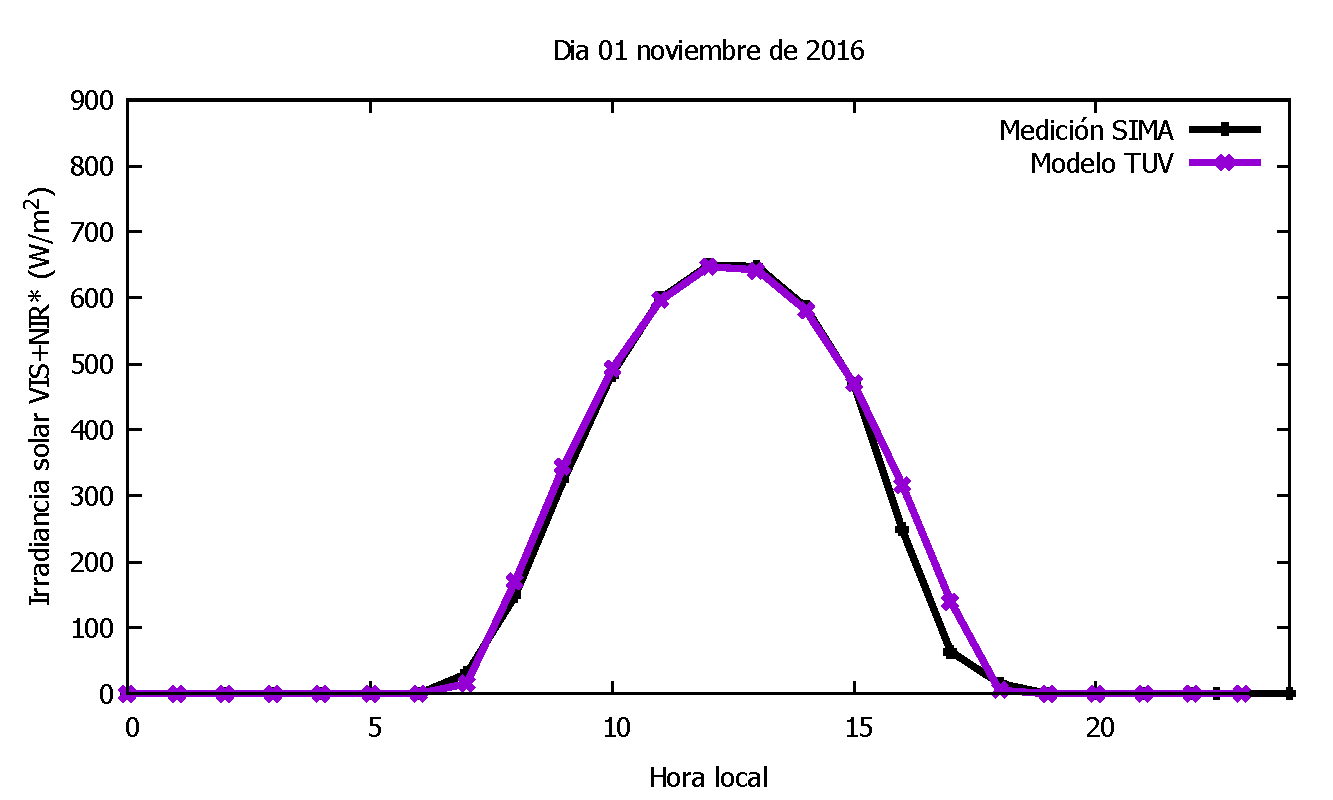
\includegraphics[scale=0.32]{images/med2.pdf}
\end{minipage}\\
\changefontsizes{10t}
\textbf{\textcolor{ver}{
Espectros solares obtenidos con SMARTS y TUV a las 13h para Estación NE el 22/feb/2015 (izq). Irradiancia solar Vis+NIR* cada hora, medida por SIMA y derivada de TUV los días 22/mar/2017 y 1/nov/2016 (der).}}
\end{minipage}
\hspace{1.2cm}
\begin{minipage}{0.45\linewidth}
\includegraphics[scale=0.43]{images/Graph4years.eps}\\
\changefontsizes{10pt} \textbf{\textcolor{ver}{
Irradiancia solar Vis+NIR* medida bajo cielo
despejado  a las 13h en Estación Noroeste y derivada de TUV y SMARTS.}}
\end{minipage}\\
\begin{minipage}{0.60\linewidth}
\begin{center}
\begin{shaded}
\textbf{\textcolor{ver}{Conclusiones}}
\end{shaded}
\end{center}
\begin{itemize}
    \item El modelo TUV5.3.2 es más eficiente para calcular la irradiancia solar $\left[400,1000\right]$nm en función del tiempo y se puede aproximar para el rango espectral del piranómetro MetOne096 del SIMA. El SMARTS2.9.5 provee la irradiancia solar $\left[400,1100\right]$nm en el mismo rango de operación del instrumento del SIMA.
    \item Conociendo principalmente el valor de aerosol en 550nm y la topografía del lugar, se puede aproximar la irradiancia solar Vis+NIR* con una DR$<$7\% entre medición y modelo. 
\end{itemize}
\end{minipage}
\hspace{1cm}\vspace{0.5cm}
\begin{minipage}{0.35\linewidth}
\begin{center}
\begin{shaded}
\textbf{\textcolor{ver}{Referencias}}
\end{shaded}
\end{center}
\changefontsizes{10pt}
\begin{enumerate}
\bibitem{Madronich} S. Madronich, Environ. UV Photob, 1-39, 1993
\bibitem{smarts} www.nrel.gov/grid/solar-resource/smarts.html.
\bibitem{tuv} https://www2.acom.ucar.edu/modeling/tropospheric-ultraviolet-and-visible-tuv-radiation-model
\bibitem{Cede} Cede A, Luccini E, Nuñez L, Piacentini R, Blumthaler M, Herman J, J.
Geophysical Research 109-D08, 2004.
\bibitem{Ipiña} Ipiña A, Salum GM, Crinó E, Piacentini R, Advances in Space
Research 966–977, 2012.
\end{enumerate}
\end{minipage}
\end{document}